\documentclass{standalone}
\usepackage{tikz}
\usetikzlibrary{patterns, positioning}


\begin{document}
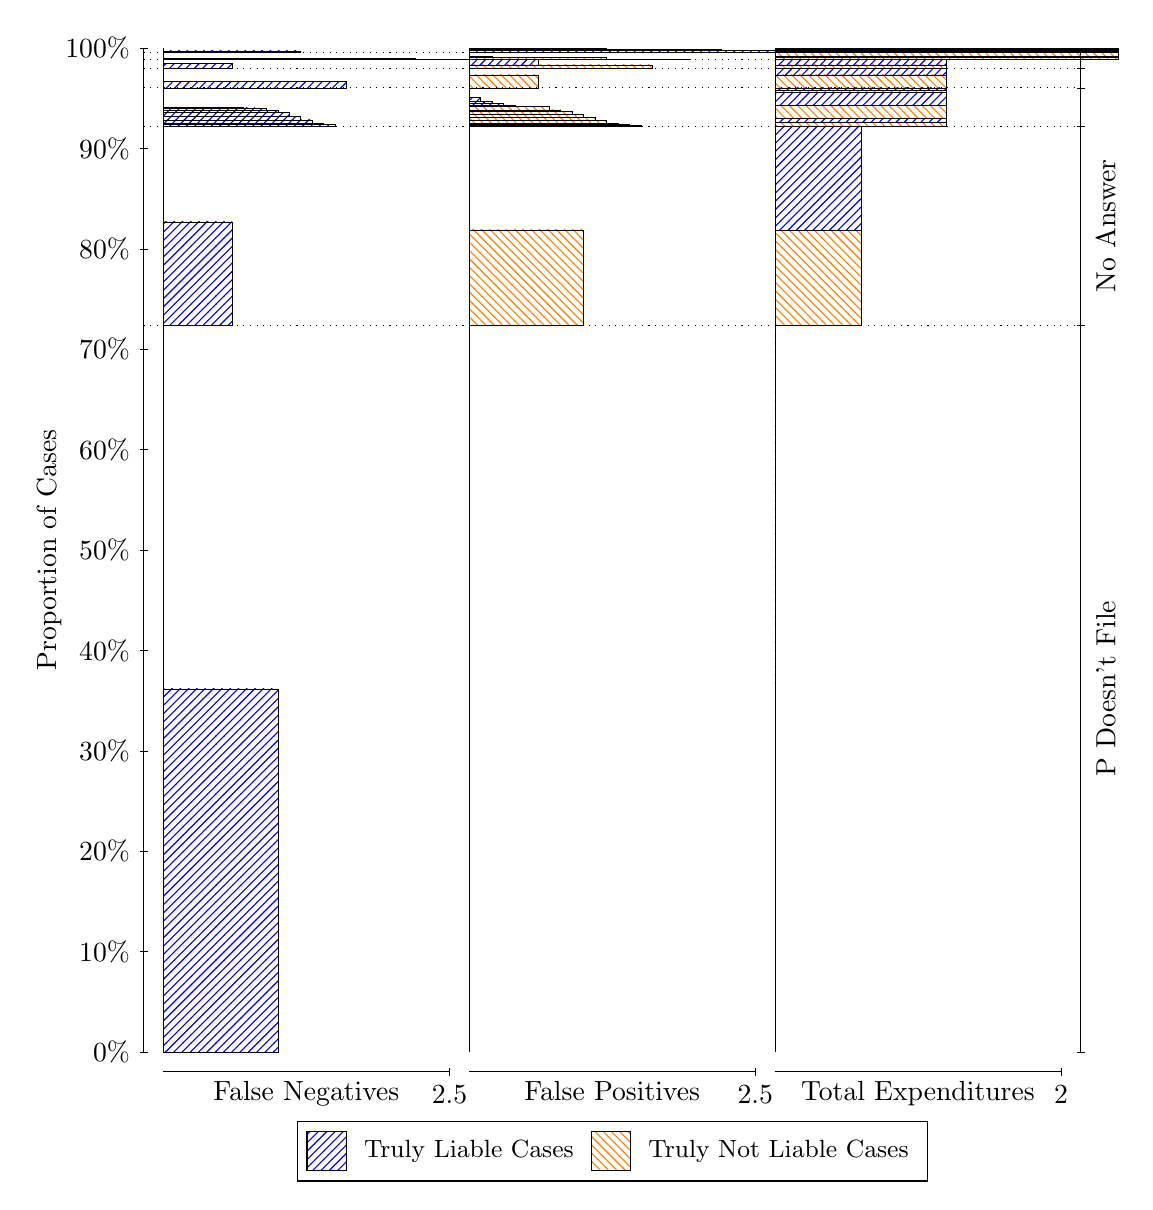
\begin{tikzpicture}
\draw[black, very thin] (1.5,1.75) -- (1.5,14.5);
\node[rotate=90, text=black, anchor=center] at (0.3, 8.125) {Proportion of Cases};
\draw[black, very thin] (1.45,1.75) -- (1.55,1.75);
\node[text=black, anchor=east] at (1.45, 1.75) {0\%};
\draw[black, very thin] (1.45,3.025) -- (1.55,3.025);
\node[text=black, anchor=east] at (1.45, 3.025) {10\%};
\draw[black, very thin] (1.45,4.3) -- (1.55,4.3);
\node[text=black, anchor=east] at (1.45, 4.3) {20\%};
\draw[black, very thin] (1.45,5.575) -- (1.55,5.575);
\node[text=black, anchor=east] at (1.45, 5.575) {30\%};
\draw[black, very thin] (1.45,6.85) -- (1.55,6.85);
\node[text=black, anchor=east] at (1.45, 6.85) {40\%};
\draw[black, very thin] (1.45,8.125) -- (1.55,8.125);
\node[text=black, anchor=east] at (1.45, 8.125) {50\%};
\draw[black, very thin] (1.45,9.4) -- (1.55,9.4);
\node[text=black, anchor=east] at (1.45, 9.4) {60\%};
\draw[black, very thin] (1.45,10.675) -- (1.55,10.675);
\node[text=black, anchor=east] at (1.45, 10.675) {70\%};
\draw[black, very thin] (1.45,11.95) -- (1.55,11.95);
\node[text=black, anchor=east] at (1.45, 11.95) {80\%};
\draw[black, very thin] (1.45,13.225) -- (1.55,13.225);
\node[text=black, anchor=east] at (1.45, 13.225) {90\%};
\draw[black, very thin] (1.45,14.5) -- (1.55,14.5);
\node[text=black, anchor=east] at (1.45, 14.5) {100\%};

\draw[black, very thin] (13.4,1.75) -- (13.4,14.5);
\draw[black, very thin] (13.35,1.75) -- (13.45,1.75);
\node[anchor=west] at (13.35, 1.75) {};
\draw[black, very thin] (13.35,10.974) -- (13.45,10.974);
\node[anchor=west] at (13.35, 10.974) {};
\draw[black, very thin] (13.35,13.508) -- (13.45,13.508);
\node[anchor=west] at (13.35, 13.508) {};
\draw[black, very thin] (13.35,13.994) -- (13.45,13.994);
\node[anchor=west] at (13.35, 13.994) {};
\draw[black, very thin] (13.35,14.241) -- (13.45,14.241);
\node[anchor=west] at (13.35, 14.241) {};
\draw[black, very thin] (13.35,14.352) -- (13.45,14.352);
\node[anchor=west] at (13.35, 14.352) {};
\draw[black, very thin] (13.35,14.446) -- (13.45,14.446);
\node[anchor=west] at (13.35, 14.446) {};
\draw[black, very thin] (13.35,14.5) -- (13.45,14.5);
\node[anchor=west] at (13.35, 14.5) {};

\draw[black, very thin, pattern color=blue, pattern=north east lines] (1.75,1.75) rectangle (3.2033,6.3621);
\draw[black, very thin, pattern color=orange, pattern=north west lines] (1.75,6.3621) rectangle (1.75,10.974);
\draw[black, very thin, pattern color=blue, pattern=north east lines] (1.75,10.974) rectangle (2.622,12.293);
\draw[black, very thin, pattern color=orange, pattern=north west lines] (1.75,12.293) rectangle (1.75,13.508);
\draw[black, very thin, pattern color=blue, pattern=north east lines] (1.75,13.508) rectangle (3.93,13.527);
\draw[black, very thin, pattern color=blue, pattern=north east lines] (1.75,13.527) rectangle (3.7847,13.542);
\draw[black, very thin, pattern color=blue, pattern=north east lines] (1.75,13.542) rectangle (3.6393,13.588);
\draw[black, very thin, pattern color=blue, pattern=north east lines] (1.75,13.588) rectangle (3.494,13.629);
\draw[black, very thin, pattern color=blue, pattern=north east lines] (1.75,13.629) rectangle (3.3487,13.682);
\draw[black, very thin, pattern color=blue, pattern=north east lines] (1.75,13.682) rectangle (3.2033,13.709);
\draw[black, very thin, pattern color=blue, pattern=north east lines] (1.75,13.709) rectangle (3.058,13.731);
\draw[black, very thin, pattern color=blue, pattern=north east lines] (1.75,13.731) rectangle (2.9127,13.739);
\draw[black, very thin, pattern color=blue, pattern=north east lines] (1.75,13.739) rectangle (2.7673,13.748);
\draw[black, very thin, pattern color=orange, pattern=north west lines] (1.75,13.748) rectangle (1.75,13.994);
\draw[black, very thin, pattern color=blue, pattern=north east lines] (1.75,13.994) rectangle (4.0753,14.078);
\draw[black, very thin, pattern color=orange, pattern=north west lines] (1.75,14.078) rectangle (1.75,14.241);
\draw[black, very thin, pattern color=blue, pattern=north east lines] (1.75,14.241) rectangle (2.622,14.307);
\draw[black, very thin, pattern color=orange, pattern=north west lines] (1.75,14.307) rectangle (1.75,14.352);
\draw[black, very thin, pattern color=blue, pattern=north east lines] (1.75,14.352) rectangle (8.4353,14.357);
\draw[black, very thin, pattern color=blue, pattern=north east lines] (1.75,14.357) rectangle (4.9473,14.366);
\draw[black, very thin, pattern color=orange, pattern=north west lines] (1.75,14.366) rectangle (1.75,14.446);
\draw[black, very thin, pattern color=blue, pattern=north east lines] (1.75,14.446) rectangle (3.494,14.465);
\draw[black, very thin, pattern color=orange, pattern=north west lines] (1.75,14.465) rectangle (1.75,14.479);
\draw[black, very thin, pattern color=blue, pattern=north east lines] (1.75,14.479) rectangle (1.75,14.5);
\draw[black, very thin, pattern color=orange, pattern=north west lines] (5.6333,1.75) rectangle (5.6333,6.3622);
\draw[black, very thin, pattern color=blue, pattern=north east lines] (5.6333,6.3622) rectangle (5.6333,10.974);
\draw[black, very thin, pattern color=orange, pattern=north west lines] (5.6333,10.974) rectangle (7.0867,12.189);
\draw[black, very thin, pattern color=blue, pattern=north east lines] (5.6333,12.189) rectangle (5.6333,13.508);
\draw[black, very thin, pattern color=orange, pattern=north west lines] (5.6333,13.508) rectangle (7.8133,13.517);
\draw[black, very thin, pattern color=orange, pattern=north west lines] (5.6333,13.517) rectangle (7.668,13.526);
\draw[black, very thin, pattern color=orange, pattern=north west lines] (5.6333,13.526) rectangle (7.5227,13.547);
\draw[black, very thin, pattern color=orange, pattern=north west lines] (5.6333,13.547) rectangle (7.3773,13.577);
\draw[black, very thin, pattern color=orange, pattern=north west lines] (5.6333,13.577) rectangle (7.232,13.623);
\draw[black, very thin, pattern color=orange, pattern=north west lines] (5.6333,13.623) rectangle (7.0867,13.659);
\draw[black, very thin, pattern color=orange, pattern=north west lines] (5.6333,13.659) rectangle (6.9413,13.7);
\draw[black, very thin, pattern color=orange, pattern=north west lines] (5.6333,13.7) rectangle (6.796,13.713);
\draw[black, very thin, pattern color=orange, pattern=north west lines] (5.6333,13.713) rectangle (6.6507,13.754);
\draw[black, very thin, pattern color=blue, pattern=north east lines] (5.6333,13.754) rectangle (6.36,13.762);
\draw[black, very thin, pattern color=blue, pattern=north east lines] (5.6333,13.762) rectangle (6.2147,13.771);
\draw[black, very thin, pattern color=blue, pattern=north east lines] (5.6333,13.771) rectangle (6.0693,13.793);
\draw[black, very thin, pattern color=blue, pattern=north east lines] (5.6333,13.793) rectangle (5.924,13.82);
\draw[black, very thin, pattern color=blue, pattern=north east lines] (5.6333,13.82) rectangle (5.7787,13.873);
\draw[black, very thin, pattern color=blue, pattern=north east lines] (5.6333,13.873) rectangle (5.6333,13.994);
\draw[black, very thin, pattern color=orange, pattern=north west lines] (5.6333,13.994) rectangle (6.5053,14.158);
\draw[black, very thin, pattern color=blue, pattern=north east lines] (5.6333,14.158) rectangle (5.6333,14.241);
\draw[black, very thin, pattern color=orange, pattern=north west lines] (5.6333,14.241) rectangle (7.9587,14.286);
\draw[black, very thin, pattern color=blue, pattern=north east lines] (5.6333,14.286) rectangle (6.5053,14.352);
\draw[black, very thin, pattern color=orange, pattern=north west lines] (5.6333,14.352) rectangle (7.3773,14.385);
\draw[black, very thin, pattern color=blue, pattern=north east lines] (5.6333,14.385) rectangle (5.924,14.394);
\draw[black, very thin, pattern color=orange, pattern=north west lines] (5.6333,14.394) rectangle (5.6333,14.442);
\draw[black, very thin, pattern color=blue, pattern=north east lines] (5.6333,14.442) rectangle (5.6333,14.446);
\draw[black, very thin, pattern color=orange, pattern=north west lines] (5.6333,14.446) rectangle (12.319,14.449);
\draw[black, very thin, pattern color=blue, pattern=north east lines] (5.6333,14.449) rectangle (10.865,14.471);
\draw[black, very thin, pattern color=orange, pattern=north west lines] (5.6333,14.471) rectangle (8.8307,14.482);
\draw[black, very thin, pattern color=blue, pattern=north east lines] (5.6333,14.482) rectangle (7.3773,14.5);
\draw[black, very thin, pattern color=orange, pattern=north west lines] (9.5167,1.75) rectangle (9.5167,6.3622);
\draw[black, very thin, pattern color=blue, pattern=north east lines] (9.5167,6.3622) rectangle (9.5167,10.974);
\draw[black, very thin, pattern color=orange, pattern=north west lines] (9.5167,10.974) rectangle (10.607,12.189);
\draw[black, very thin, pattern color=blue, pattern=north east lines] (9.5167,12.189) rectangle (10.607,13.508);
\draw[black, very thin, pattern color=orange, pattern=north west lines] (9.5167,13.508) rectangle (11.697,13.553);
\draw[black, very thin, pattern color=blue, pattern=north east lines] (9.5167,13.553) rectangle (11.697,13.606);
\draw[black, very thin, pattern color=orange, pattern=north west lines] (9.5167,13.606) rectangle (11.697,13.776);
\draw[black, very thin, pattern color=blue, pattern=north east lines] (9.5167,13.776) rectangle (11.697,13.933);
\draw[black, very thin, pattern color=orange, pattern=north west lines] (9.5167,13.933) rectangle (11.697,13.964);
\draw[black, very thin, pattern color=blue, pattern=north east lines] (9.5167,13.964) rectangle (11.697,13.994);
\draw[black, very thin, pattern color=orange, pattern=north west lines] (9.5167,13.994) rectangle (11.697,14.158);
\draw[black, very thin, pattern color=blue, pattern=north east lines] (9.5167,14.158) rectangle (11.697,14.241);
\draw[black, very thin, pattern color=orange, pattern=north west lines] (9.5167,14.241) rectangle (11.697,14.286);
\draw[black, very thin, pattern color=blue, pattern=north east lines] (9.5167,14.286) rectangle (11.697,14.352);
\draw[black, very thin, pattern color=orange, pattern=north west lines] (9.5167,14.352) rectangle (13.877,14.385);
\draw[black, very thin, pattern color=blue, pattern=north east lines] (9.5167,14.385) rectangle (13.877,14.394);
\draw[black, very thin, pattern color=orange, pattern=north west lines] (9.5167,14.394) rectangle (13.877,14.442);
\draw[black, very thin, pattern color=blue, pattern=north east lines] (9.5167,14.442) rectangle (13.877,14.446);
\draw[black, very thin, pattern color=orange, pattern=north west lines] (9.5167,14.446) rectangle (13.877,14.457);
\draw[black, very thin, pattern color=blue, pattern=north east lines] (9.5167,14.457) rectangle (13.877,14.476);
\draw[black, very thin, pattern color=orange, pattern=north west lines] (9.5167,14.476) rectangle (13.877,14.479);
\draw[black, very thin, pattern color=blue, pattern=north east lines] (9.5167,14.479) rectangle (13.877,14.5);
\draw[black, dotted] (1.5,10.974) -- (13.4,10.974);
\draw[black, dotted] (1.5,13.508) -- (13.4,13.508);
\draw[black, dotted] (1.5,13.994) -- (13.4,13.994);
\draw[black, dotted] (1.5,14.241) -- (13.4,14.241);
\draw[black, dotted] (1.5,14.352) -- (13.4,14.352);
\draw[black, dotted] (1.5,14.446) -- (13.4,14.446);
\draw[black, very thin] (1.75,1.5) -- (5.3833,1.5);
\node[text=black, anchor=north] at (3.5667, 1.5) {False Negatives};
\draw[black, very thin] (5.3833,1.45) -- (5.3833,1.55);
\node[text=black, anchor=north] at (5.3833, 1.45) {2.5};

\draw[black, very thin] (5.6333,1.5) -- (9.2667,1.5);
\node[text=black, anchor=north] at (7.45, 1.5) {False Positives};
\draw[black, very thin] (9.2667,1.45) -- (9.2667,1.55);
\node[text=black, anchor=north] at (9.2667, 1.45) {2.5};

\draw[black, very thin] (9.5167,1.5) -- (13.15,1.5);
\node[text=black, anchor=north] at (11.333, 1.5) {Total Expenditures};
\draw[black, very thin] (13.15,1.45) -- (13.15,1.55);
\node[text=black, anchor=north] at (13.15, 1.45) {2};

\node[text=black, centered, rotate=90] at (13.72, 6.3621) {P Doesn't File};
\node[text=black, centered, rotate=90] at (13.72, 12.241) {No Answer};






\draw (7.449999999999999,1.5) node[draw=none] (baseCoordinate) {};
\begin{scope}[align=center]
        \matrix[scale=0.5, draw=black, below=0.5cm of baseCoordinate, nodes={draw}, column sep=0.1cm]{
            \node[rectangle, draw, minimum width=0.5cm, minimum height=0.5cm, pattern color=blue, pattern=north east lines] {}; &
            \node[draw=none, font=\small, text=black] (B) {Truly Liable Cases}; &
            \node[rectangle, draw, minimum width=0.5cm, minimum height=0.5cm, pattern color=orange, pattern=north west lines] {}; &
            \node[draw=none, font=\small, text=black] (B) {Truly Not Liable Cases}; \\
            };
\end{scope}

\end{tikzpicture}
\end{document}